% eec_v0_relation.tex -- note: mathematical relation between energy-energy
% correlators and the jet--UE v0(pT). Figures: make_figs.py (schematic only).
\documentclass[11pt,a4paper]{article}
\usepackage[margin=2.3cm]{geometry}
\usepackage{amsmath,amssymb,bm}
\usepackage{graphicx}
\usepackage{booktabs}
\usepackage[numbers,sort&compress]{natbib}
\usepackage[colorlinks=true,linkcolor=blue,citecolor=blue,urlcolor=blue]{hyperref}

\newcommand{\pT}{p_\mathrm{T}}
\newcommand{\vjet}{v_0^{\mathrm{jet\text{-}UE}}}
\newcommand{\mpt}{[\pT]_\mathrm{ref}}
\newcommand{\Ctwo}{C_{2,\mathrm{ref}}}
\newcommand{\K}{\mathcal{K}_R}
\newcommand{\Rr}{\mathcal{R}_R}
\newcommand{\Nref}{N_\mathrm{ref}}
\newcommand{\pjet}{p_\mathrm{T}^\mathrm{jet}}

\title{Energy--energy correlators and the jet--UE $v_0(\pT)$:\\ the mathematical relation}
\author{Somadutta Bhatta}
\date{\today}

\begin{document}
\maketitle

\begin{abstract}
\noindent
We write the jet--underlying-event (UE) observable $\vjet(\pT)$ and the energy--energy correlators (EECs) in terms of one function, the connected two-particle density $C(x_1,x_2)$. Both are linear functionals of $C$. The jet--UE EEC weights a pair by $p_{\mathrm{T},1}\,p_{\mathrm{T},2}$ and keeps the angle. The covariance in $\vjet$ weights the in-cone particle by a shape projector and the reference particle by $p_{\mathrm{T},2}-\mu$, and integrates the angle over the reference region. Two angular kernels, $\Gamma_0$ and $\Gamma_1$, contain everything both observables need. The relation is exact for the EEC and holds to leading order in event-by-event fluctuations for $\vjet$. The note contains only the definitions, the derivation and the conditions under which the relation holds.
\end{abstract}

\begin{figure}[h]
\centering
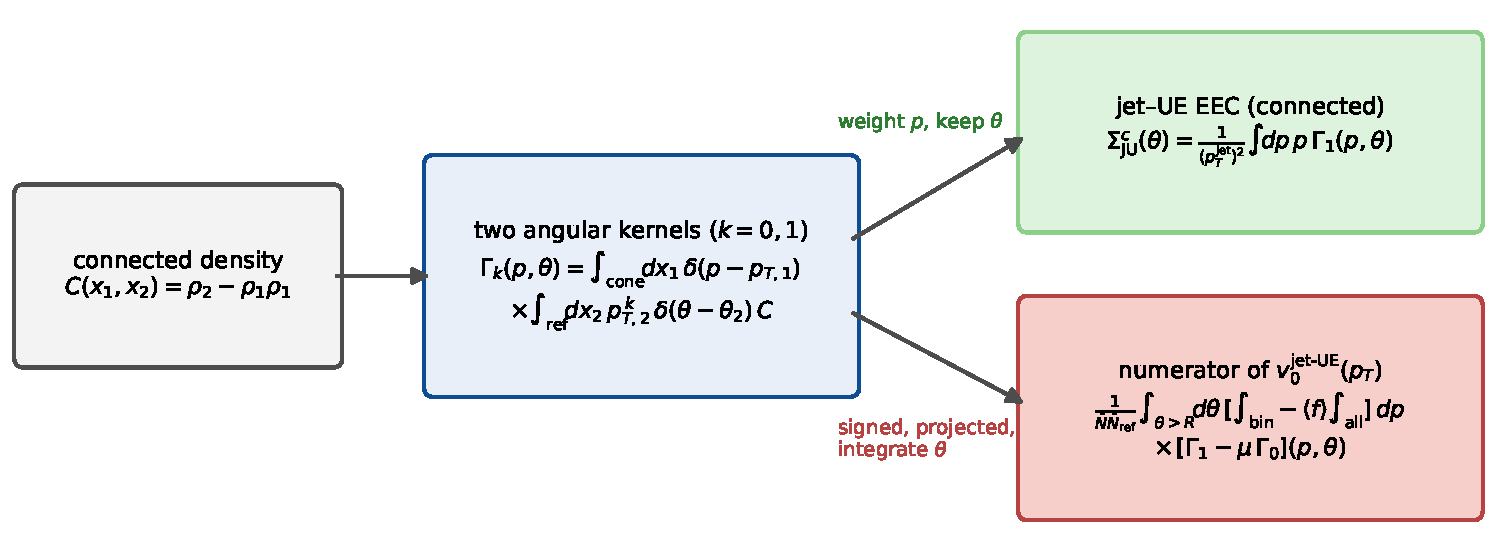
\includegraphics[width=\textwidth]{figs/fig4_flow.pdf}
\caption{Overview. Both observables are built from the connected density $C$ of one particle in the jet cone ($x_1$) and one in the reference region ($x_2$). The two kernels $\Gamma_0$ and $\Gamma_1$ (Eq.~\ref{eq:gamma}) contain everything that either observable uses. The jet--UE EEC (Eq.~\ref{eq:eec_gamma}) and the numerator of $\vjet$ (Eq.~\ref{eq:cov_gamma}) take different weighted integrals of them.}
\label{fig:flow}
\end{figure}

%------------------------------------------------------------------------------
\section{Notation}
\label{sec:notation}

\paragraph{Particles and regions.}
Each event contains one leading jet. A charged particle is written $x=(\pT,\eta,\varphi)$, with $\eta$ and $\varphi$ measured relative to the jet axis, and $\theta(x)=\sqrt{\Delta\eta^2+\Delta\varphi^2}$ is its angle to the axis. Two regions are used (Fig.~\ref{fig:geometry}):
\begin{itemize}
\item the jet cone $\K=\{x:\theta(x)<R\}$;
\item the reference region $\Rr$: $0.2<\pT<3$~GeV/$c$, inside the tracking acceptance, with $\theta(x)>R$, and outside the two perpendicular cones.
\end{itemize}
The two regions are disjoint. We write $\mathbf{1}_A(x)$ for the indicator of a region $A$, and $\chi_b(x)$ for the indicator that $\pT$ lies in probe bin $b$.

\paragraph{Densities.}
With $\langle\cdot\rangle$ the average over events,
\begin{align}
\rho_1(x) &= \Big\langle \sum_i \delta(x-x_i)\Big\rangle, \qquad
\rho_2(x_1,x_2) = \Big\langle \sum_{i\neq j} \delta(x_1-x_i)\,\delta(x_2-x_j)\Big\rangle,\\
C(x_1,x_2) &= \rho_2(x_1,x_2)-\rho_1(x_1)\,\rho_1(x_2).
\label{eq:C}
\end{align}
$C$ is the connected (two-particle-correlated) part of the pair density. It vanishes for pairs of particles that are statistically independent.

\paragraph{One identity.}
For any two additive event quantities $A=\sum_i a(x_i)$ and $B=\sum_j b(x_j)$,
\begin{equation}
\langle A\rangle=\int\!dx\,a(x)\,\rho_1(x),\qquad
\mathrm{Cov}(A,B)=\int\!dx_1\!\int\!dx_2\;a(x_1)\,b(x_2)\,C(x_1,x_2)\;+\;\int\!dx\;a(x)\,b(x)\,\rho_1(x).
\label{eq:covid}
\end{equation}
The last term counts a particle paired with itself (App.~\ref{app:covid}). It vanishes when $a$ and $b$ have disjoint support, which is the case for every jet--reference pair below.

\begin{figure}[t]
\centering
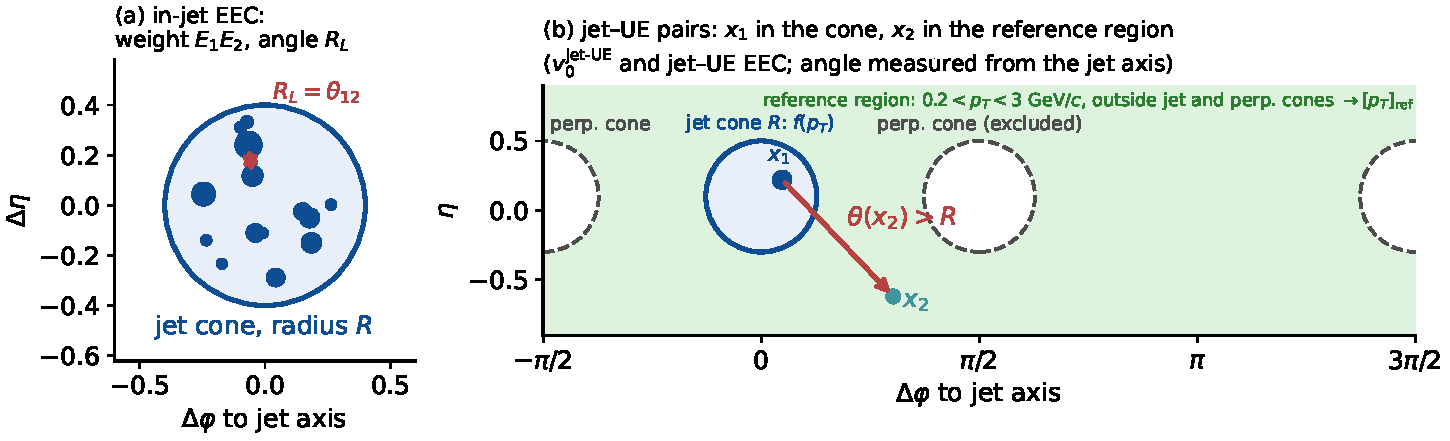
\includegraphics[width=\textwidth]{figs/fig1_geometry.pdf}
\caption{Regions and pairs. (a)~The in-jet EEC pairs two particles inside the jet and resolves their separation $R_L$. (b)~The jet--UE pairs used here: $x_1$ in the cone $\K$ and $x_2$ in the reference region $\Rr$ (shaded, outside the cone and the perpendicular cones). The angle $\theta(x_2)$ of $x_2$ to the jet axis is always larger than $R$.}
\label{fig:geometry}
\end{figure}

%------------------------------------------------------------------------------
\section{The two observables}
\label{sec:defs}

\paragraph{$\vjet$.}
The in-cone yield in bin $b$, the in-cone multiplicity, and the reference sums are
\begin{equation}
n_b=\sum_i \mathbf{1}_{\K}(x_i)\,\chi_b(x_i),\quad N=\sum_i\mathbf{1}_{\K}(x_i),\quad
S=\sum_j \mathbf{1}_{\Rr}(x_j)\,p_{\mathrm{T},j},\quad \Nref=\sum_j\mathbf{1}_{\Rr}(x_j).
\end{equation}
The probe is $f_b=n_b/N$ and the reference is $\mpt=S/\Nref$. With $\mu=\langle\mpt\rangle$,
\begin{equation}
\vjet(b)=\frac{\mathrm{Cov}\big(f_b,\mpt\big)}{\langle f_b\rangle\sqrt{\Ctwo}},\qquad
\Ctwo=\big\langle (p_{\mathrm{T},i}-\mu)(p_{\mathrm{T},j}-\mu)\big\rangle_{i\neq j\in\Rr}.
\label{eq:v0}
\end{equation}
This follows the $v_0(\pT)$ construction for bulk particles~\cite{Schenke:2020uqq,ATLAS:2025v0pt,ALICE:2025v0pt}. Since $\sum_b f_b=1$ in every event, $\sum_b\mathrm{Cov}(f_b,\mpt)=0$.

\paragraph{Energy--energy correlators.}
For jets in a narrow $\pjet$ class, the in-jet EEC is
\begin{align}
\Sigma_\mathrm{J}(R_L)&=\frac{1}{(\pjet)^2}\Big\langle\sum_{i\neq j\in\K}p_{\mathrm{T},i}\,p_{\mathrm{T},j}\;\delta(R_L-\Delta_{ij})\Big\rangle\nonumber\\
&=\frac{1}{(\pjet)^2}\int_{\K}\!dx_1\!\int_{\K}\!dx_2\;p_{\mathrm{T},1}\,p_{\mathrm{T},2}\;\delta(R_L-\Delta_{12})\,\rho_2(x_1,x_2),
\label{eq:eecJ}
\end{align}
with $\Delta_{ij}$ the pair separation~\cite{Basham:1978bw,Andres:2022ovj}. The jet--UE EEC pairs a jet particle with a reference particle and records the angle of the reference particle to the axis. Its connected version subtracts uncorrelated pairs (in practice with mixed events from the same event class), which replaces $\rho_2$ by $C$:
\begin{equation}
\Sigma^{c}_\mathrm{JU}(\theta)=\frac{1}{(\pjet)^2}\int_{\K}\!dx_1\!\int_{\Rr}\!dx_2\;p_{\mathrm{T},1}\,p_{\mathrm{T},2}\;\delta\big(\theta-\theta(x_2)\big)\,C(x_1,x_2).
\label{eq:eecJU}
\end{equation}
Another choice records the pair separation $\Delta_{12}$ instead of $\theta(x_2)$. This changes only the angular variable, and $\vjet$ integrates over the angle in any case (Sec.~\ref{sec:R}).

%------------------------------------------------------------------------------
\section{The common kernel}
\label{sec:kernel}

Define, for an in-cone momentum $p$ and a reference angle $\theta$,
\begin{equation}
\Gamma_k(p,\theta)=\int_{\K}\!dx_1\;\delta(p-p_{\mathrm{T},1})\int_{\Rr}\!dx_2\;p_{\mathrm{T},2}^{\,k}\;\delta\big(\theta-\theta(x_2)\big)\;C(x_1,x_2),\qquad k=0,1 .
\label{eq:gamma}
\end{equation}
$\Gamma_0$ is the connected correlation between the number of in-cone particles at momentum $p$ and the number of reference particles at angle $\theta$. $\Gamma_1$ is the same correlation with the reference particles weighted by their momentum. Their ratio $\Gamma_1/\Gamma_0$ is the mean momentum of the correlated reference particles at that $(p,\theta)$.

\subsection{The jet--UE EEC}
Integrating Eq.~(\ref{eq:eecJU}) over $x_1$ at fixed $p_{\mathrm{T},1}=p$ gives directly
\begin{equation}
\boxed{\;\Sigma^{c}_\mathrm{JU}(\theta)=\frac{1}{(\pjet)^2}\int\!dp\;p\;\Gamma_1(p,\theta)\;}
\label{eq:eec_gamma}
\end{equation}
This is exact, because the EEC is already linear in the pair density. Only $\Gamma_1$ enters, weighted by the in-cone momentum $p$ and resolved in $\theta$.

\subsection{The covariance in $\vjet$}
\paragraph{Linearization.}
Write every count as mean plus fluctuation, $n_b=\bar n_b+\delta n_b$, $N=\bar N+\delta N$, $S=\bar S+\delta S$, $\Nref=\bar N_\mathrm{ref}+\delta\Nref$, and define $\bar f_b=\bar n_b/\bar N$ and $\bar\mu=\bar S/\bar N_\mathrm{ref}$. To first order in the fluctuations,
\begin{equation}
f_b-\bar f_b\simeq\frac{\delta n_b-\bar f_b\,\delta N}{\bar N},\qquad
\mpt-\bar\mu\simeq\frac{\delta S-\bar\mu\,\delta\Nref}{\bar N_\mathrm{ref}},
\end{equation}
so
\begin{equation}
\mathrm{Cov}(f_b,\mpt)\simeq\frac{1}{\bar N\,\bar N_\mathrm{ref}}\,
\mathrm{Cov}\Big(n_b-\bar f_b N,\;S-\bar\mu\,\Nref\Big).
\label{eq:lin}
\end{equation}
The neglected terms are third-order moments of the fluctuations, such as $\langle\delta n_b\,\delta N\,\delta S\rangle/(\bar N^2\bar N_\mathrm{ref})$. For Poisson-like fluctuations they are suppressed by $1/\bar N$ or $1/\bar N_\mathrm{ref}$ relative to the leading term. Also, $\mu=\langle S/\Nref\rangle$ and $\bar\mu=\langle S\rangle/\langle\Nref\rangle$ differ only at this order.

\paragraph{Correlator form.}
Both arguments in Eq.~(\ref{eq:lin}) are additive:
\begin{equation}
n_b-\bar f_b N=\sum_i \mathbf{1}_{\K}(x_i)\big[\chi_b(x_i)-\bar f_b\big],\qquad
S-\bar\mu\,\Nref=\sum_j \mathbf{1}_{\Rr}(x_j)\big[p_{\mathrm{T},j}-\bar\mu\big].
\end{equation}
The two supports are disjoint, so Eq.~(\ref{eq:covid}) has no self term, and
\begin{equation}
\mathrm{Cov}(f_b,\mpt)\simeq\frac{1}{\bar N\,\bar N_\mathrm{ref}}
\int_{\K}\!dx_1\!\int_{\Rr}\!dx_2\;
\underbrace{\big[\chi_b(x_1)-\bar f_b\big]}_{w_\mathrm{J}(x_1)}\;
\underbrace{\big[p_{\mathrm{T},2}-\bar\mu\big]}_{w_\mathrm{R}(x_2)}\;C(x_1,x_2).
\label{eq:cov_C}
\end{equation}
In terms of the kernels of Eq.~(\ref{eq:gamma}),
\begin{equation}
\boxed{\;\mathrm{Cov}(f_b,\mpt)\simeq\frac{1}{\bar N\,\bar N_\mathrm{ref}}\int_{\Rr}\!d\theta\;
\Big[\int_{b}\!dp-\bar f_b\!\int\!dp\Big]\;\big(\Gamma_1-\bar\mu\,\Gamma_0\big)(p,\theta)\;}
\label{eq:cov_gamma}
\end{equation}
where $\int_b dp$ runs over probe bin $b$ and $\int dp$ over all in-cone momenta.

\subsection{The normalization $\Ctwo$}
$\Ctwo$ is a reference--reference moment of the same $C$. In the pair-weighted form,
\begin{align}
\Ctwo&=\frac{\int_{\Rr}\!dx_1\int_{\Rr}\!dx_2\,(p_{\mathrm{T},1}-\bar\mu)(p_{\mathrm{T},2}-\bar\mu)\,\rho_2}{\langle\Nref(\Nref-1)\rangle}
=\frac{\Lambda}{\langle\Nref(\Nref-1)\rangle},\label{eq:c2}\\
\Lambda&\equiv\int_{\Rr}\!dx_1\int_{\Rr}\!dx_2\,(p_{\mathrm{T},1}-\bar\mu)(p_{\mathrm{T},2}-\bar\mu)\,C(x_1,x_2).\nonumber
\end{align}
Here $\rho_2$ can be replaced by $C$ because $\int_{\Rr}(\pT-\bar\mu)\rho_1=\langle S\rangle-\bar\mu\langle\Nref\rangle=0$. The event-weighted definition used in practice differs from the pair-weighted one at the order of Eq.~(\ref{eq:lin}).

\subsection{All of $\vjet$ in terms of $C$}
Combining Eqs.~(\ref{eq:cov_C}) and (\ref{eq:c2}), and using $\bar N\bar f_b=\bar n_b$,
\begin{equation}
\boxed{\;\vjet(b)\simeq\frac{M_b}{\bar n_b\,\sqrt{\Lambda}}\;\frac{\sqrt{\langle\Nref(\Nref-1)\rangle}}{\bar N_\mathrm{ref}},\qquad
M_b=\int_{\K}\!\int_{\Rr}\big[\chi_b(x_1)-\bar f_b\big]\big[p_{\mathrm{T},2}-\bar\mu\big]\,C\;}
\label{eq:v0_C}
\end{equation}
The last factor equals $1$ up to terms of order $\mathrm{Var}(\Nref)/\bar N_\mathrm{ref}^2-1/\bar N_\mathrm{ref}$. So $\vjet$ is a jet--reference moment of $C$ divided by the in-cone yield and by the square root of a reference--reference moment of the same $C$.

%------------------------------------------------------------------------------
\section{The relation}
\label{sec:relation}

\paragraph{Same density, different weights.}
Define a general weighted jet--reference correlator
\begin{equation}
\Sigma[a,b](\theta)=\int_{\K}\!dx_1\!\int_{\Rr}\!dx_2\;a(x_1)\,b(x_2)\,\delta\big(\theta-\theta(x_2)\big)\,C(x_1,x_2).
\end{equation}
Then
\begin{equation}
\Sigma^{c}_\mathrm{JU}(\theta)=\Sigma\Big[\tfrac{p_{\mathrm{T},1}}{\pjet},\tfrac{p_{\mathrm{T},2}}{\pjet}\Big](\theta),\qquad
\mathrm{Cov}(f_b,\mpt)\simeq\frac{1}{\bar N\bar N_\mathrm{ref}}\int_{\Rr}\!d\theta\;\Sigma\big[\chi_b-\bar f_b,\;p_{\mathrm{T},2}-\bar\mu\big](\theta).
\label{eq:relation}
\end{equation}
The covariance in $\vjet$ is therefore the angle-integrated jet--UE EEC with two weight replacements (Table~\ref{tab:compare} and Fig.~\ref{fig:weights}):
\begin{itemize}
\item jet side: $p_{\mathrm{T},1}/\pjet\;\to\;\chi_b(x_1)-\bar f_b$, which selects one in-cone bin and subtracts its share of the total in-cone yield;
\item reference side: $p_{\mathrm{T},2}/\pjet\;\to\;p_{\mathrm{T},2}-\bar\mu$, the momentum relative to the reference mean, which can have either sign.
\end{itemize}

\begin{figure}[t]
\centering
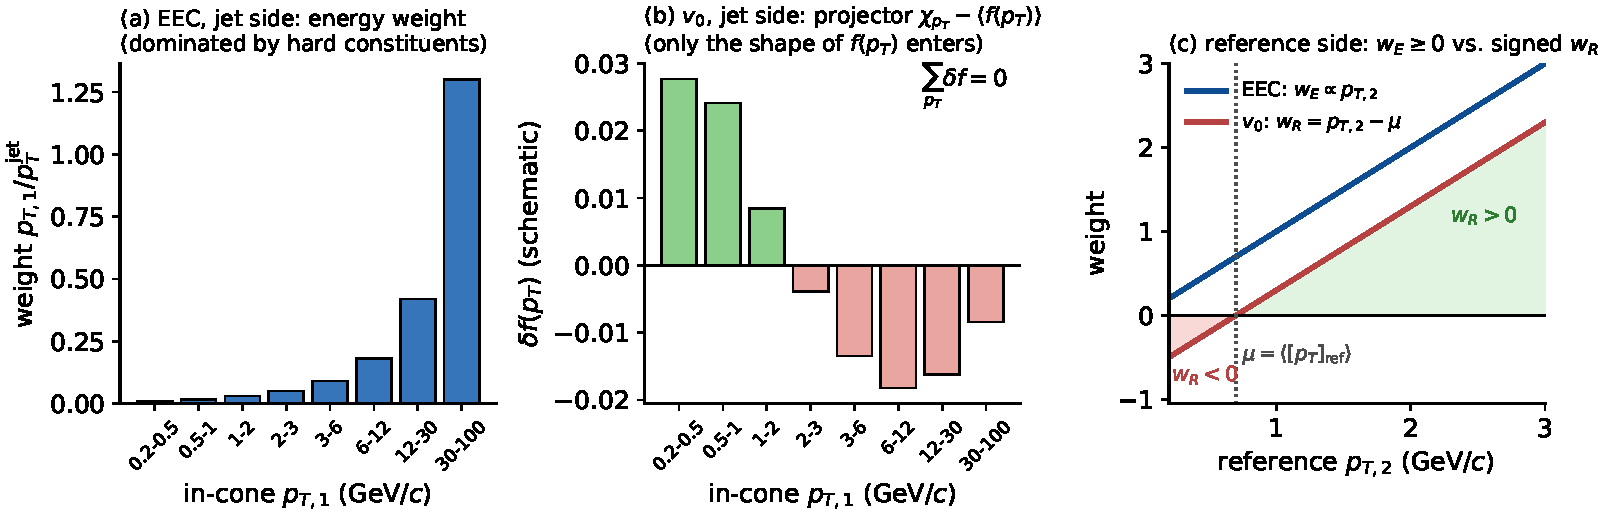
\includegraphics[width=\textwidth]{figs/fig2_weights.pdf}
\caption{The weights of Eq.~(\ref{eq:relation}). (a)~EEC, jet side: $p_{\mathrm{T},1}/\pjet$. (b)~$\vjet$, jet side: the projector $\chi_b-\bar f_b$. Only changes of the shape of $f(\pT)$ contribute, and the contributions of all bins sum to zero (shown for an illustrative shape change). (c)~Reference side: the EEC weight $p_{\mathrm{T},2}$ is positive; the $\vjet$ weight $p_{\mathrm{T},2}-\bar\mu$ changes sign at $\bar\mu$.}
\label{fig:weights}
\end{figure}

\begin{table}[t]
\centering
\caption{Term-by-term comparison of the two observables as functionals of $C$.}
\label{tab:compare}
\begin{tabular}{lll}
\toprule
 & jet--UE EEC, $\Sigma^{c}_\mathrm{JU}(\theta)$ & numerator of $\vjet(b)$\\
\midrule
pair region & $x_1\in\K$, $x_2\in\Rr$ & $x_1\in\K$, $x_2\in\Rr$\\
density & $C$ (after mixed-event subtraction) & $C$ (from the covariance)\\
jet-side weight & $p_{\mathrm{T},1}/\pjet\geq0$ & $\chi_b(x_1)-\bar f_b$ (projector, $\sum_b=0$)\\
reference-side weight & $p_{\mathrm{T},2}/\pjet\geq0$ & $p_{\mathrm{T},2}-\bar\mu$ (signed)\\
kernels used & $\Gamma_1$ & $\Gamma_1-\bar\mu\,\Gamma_0$\\
angle & resolved, $\theta$ & integrated over $\Rr$ ($\theta>R$)\\
normalization & $(\pjet)^{-2}$ per jet & $\bar n_b^{-1}\Lambda^{-1/2}$ (Eq.~\ref{eq:v0_C})\\
validity & exact & leading order in fluctuations\\
\bottomrule
\end{tabular}
\end{table}

\paragraph{What one observable fixes about the other.}
Let $G_b\equiv\int_{\Rr}d\theta\int_b dp\,(\Gamma_1-\bar\mu\Gamma_0)$. The set of covariances $M_b$ over all bins is $M=(\mathsf{I}-\bar{\bm f}\,\bm 1^{\mathsf T})\,G$, where $\bar{\bm f}$ is the vector of $\bar f_b$. Since $\sum_b\bar f_b=1$, this map has a one-dimensional null space, $G\propto\bar{\bm f}$. Therefore:
\begin{enumerate}
\item $\vjet$ over all bins determines $G_b$ up to an additive term proportional to $\bar f_b$. The part of the jet--UE correlation that only changes the total in-cone multiplicity, with the in-cone spectrum shape unchanged, is invisible to $\vjet$. This is the sum rule $\sum_b M_b=0$.
\item $\vjet$ does not determine $\Sigma^c_\mathrm{JU}(\theta)$. That would need $\Gamma_1$ alone (not $\Gamma_1-\bar\mu\Gamma_0$), its angular dependence, and the projected-out part.
\item $\Sigma^c_\mathrm{JU}(\theta)$ does not determine $\vjet$. That would need $\Gamma_0$, the in-cone momentum dependence of $\Gamma_1$ (not only its $p$-weighted integral), and the normalization $\Lambda$.
\item Both are fixed if $\Gamma_0(p,\theta)$ and $\Gamma_1(p,\theta)$ are known, together with $\Lambda$ and the mean counts $\bar n_b$ and $\bar N_\mathrm{ref}$.
\end{enumerate}
The in-jet EEC, Eq.~(\ref{eq:eecJ}), uses pairs with both particles in $\K$. $\vjet$ contains no such pairs, so no relation exists between $\vjet$ and the in-jet EEC beyond the fact that both are moments of $\rho_2$ in different regions.

%------------------------------------------------------------------------------
\section{Angle and radius}
\label{sec:R}

\begin{figure}[t]
\centering
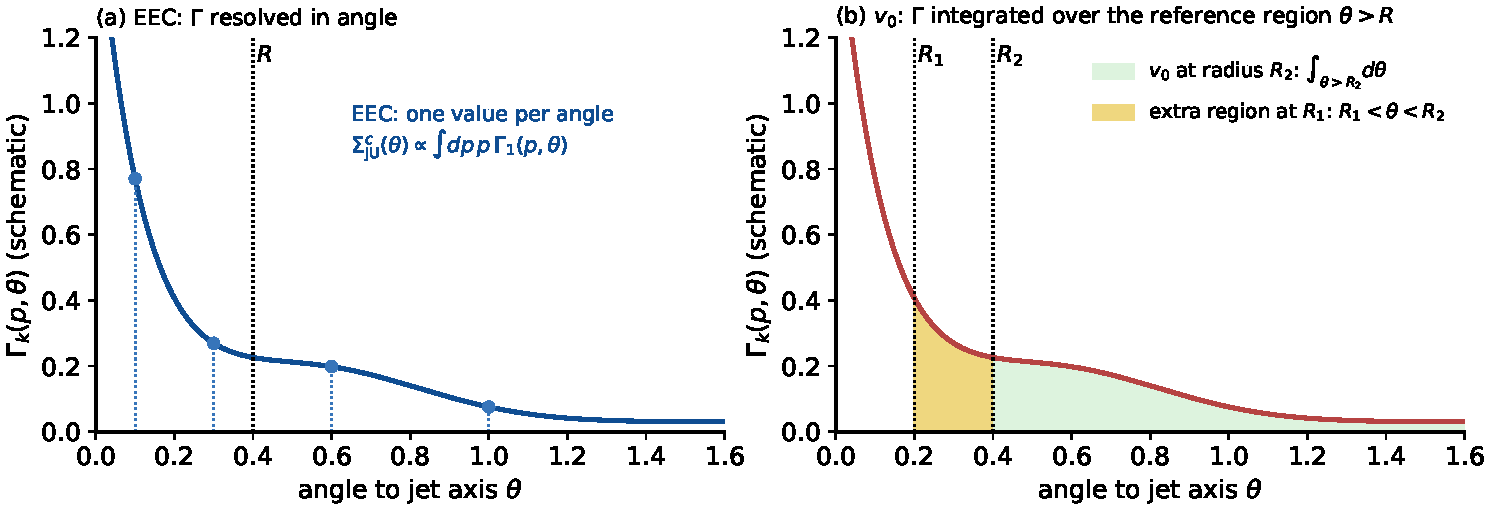
\includegraphics[width=\textwidth]{figs/fig3_angle.pdf}
\caption{Angular treatment (schematic kernel). (a)~The EEC records $\Gamma$ angle by angle. (b)~$\vjet$ at radius $R$ integrates $\Gamma$ over the reference region, $\theta>R$. Going from $R_2$ to a smaller $R_1$ adds the band $R_1<\theta<R_2$ to the reference side. At the same time the cone shrinks, so the jet side changes as well (Eq.~\ref{eq:dR}).}
\label{fig:angle}
\end{figure}

$\vjet$ has no angular variable of its own. The angle enters only through the region boundaries $\K$ and $\Rr$, and both move with $R$. For two radii $R_1<R_2$ the numerators differ by
\begin{equation}
M_b(R_2)-M_b(R_1)=
\underbrace{\int_{\mathcal{K}_{R_2}\setminus\mathcal{K}_{R_1}}\!\int_{\mathcal{R}_{R_2}}w_\mathrm{J}w_\mathrm{R}\,C}_{\text{jet side gains }R_1<\theta_1<R_2}
\;-\;\underbrace{\int_{\mathcal{K}_{R_1}}\!\int_{\mathcal{R}_{R_1}\setminus\mathcal{R}_{R_2}}w_\mathrm{J}w_\mathrm{R}\,C}_{\text{reference side loses }R_1<\theta_2<R_2}
\;+\;\Delta_{w},
\label{eq:dR}
\end{equation}
where the weights $w_\mathrm{J},w_\mathrm{R}$ are held fixed in the two integrals and $\Delta_w$ collects the change of the weights themselves ($\bar f_b$ and $\bar\mu$ depend on $R$). Since $\mathcal{R}_{R_2}\subset\mathcal{R}_{R_1}$, the set $\mathcal{R}_{R_1}\setminus\mathcal{R}_{R_2}$ is the band $R_1<\theta<R_2$ together with the rings by which the perpendicular cones grow. A difference between two radii is therefore not a pure angular slice of $\Gamma$ at fixed jet side, unlike $\Sigma^{c}_\mathrm{JU}(\theta)$ at two angles. It becomes one only if the jet-side change (first term) and $\Delta_w$ are negligible.

Because $\vjet$ integrates over $\Rr$, the same expression results whether the kernel is written in the angle to the axis $\theta(x_2)$ or in the pair separation $\Delta_{12}$. Only the region boundaries matter.

%------------------------------------------------------------------------------
\section{Conditions for the relation}
\label{sec:conditions}

\begin{enumerate}
\item \emph{Same regions.} Equation~(\ref{eq:relation}) compares the two observables with the same $\K$ and $\Rr$: the same reference momentum window, the same $\eta$ acceptance and the same perpendicular-cone exclusion. A jet--UE EEC measured in a different region is a different integral of $C$.
\item \emph{Disjoint regions.} No particle may enter both the cone and the reference, otherwise a self term $\int a\,b\,\rho_1$ appears (Eq.~\ref{eq:covid}).
\item \emph{Leading order.} The $\vjet$ side holds to first order in the fluctuations of the counts (Eq.~\ref{eq:lin}). The EEC side is exact.
\item \emph{Event class.} Both $C$'s are defined in the same event and jet selection. For the EEC this means that the mixed-event pairs come from the same class, so that the subtraction removes exactly $\rho_1\rho_1$.
\item \emph{Normalizations.} The EEC is normalized per jet by $(\pjet)^2$; for a finite $\pjet$ class this factor sits inside the average. $\vjet$ is normalized by $\bar n_b\sqrt\Lambda$ and is independent of $\pjet$ except through the jet selection.
\end{enumerate}

%------------------------------------------------------------------------------
\appendix
\section{Proof of Eq.~(\ref{eq:covid})}
\label{app:covid}
$\langle AB\rangle=\big\langle\sum_{i,j}a(x_i)b(x_j)\big\rangle=\big\langle\sum_{i\neq j}a(x_i)b(x_j)\big\rangle+\big\langle\sum_i a(x_i)b(x_i)\big\rangle
=\int\!\!\int a\,b\,\rho_2+\int a\,b\,\rho_1$, and $\langle A\rangle\langle B\rangle=\int\!\!\int a\,b\,\rho_1\rho_1$. Subtracting gives Eq.~(\ref{eq:covid}).

\section{From Eq.~(\ref{eq:cov_C}) to Eq.~(\ref{eq:cov_gamma})}
Insert $1=\int dp\,\delta(p-p_{\mathrm{T},1})$ and $1=\int d\theta\,\delta(\theta-\theta(x_2))$ into Eq.~(\ref{eq:cov_C}). Then $\chi_b(x_1)$ restricts $p$ to bin $b$, and $p_{\mathrm{T},2}-\bar\mu$ splits into the $k=1$ and $k=0$ kernels of Eq.~(\ref{eq:gamma}). The same insertion in Eq.~(\ref{eq:eecJU}) with $p_{\mathrm{T},1}\to p$ gives Eq.~(\ref{eq:eec_gamma}).

\bibliographystyle{unsrtnat}
\bibliography{refs_eec_note}

\end{document}
